\documentclass[11pt,letterpaper,twoside,english]{article}

\usepackage[margin=1.4in]{geometry} % controls the size of the margins

% Special symbols, etc.
\usepackage{amssymb,amsbsy,latexsym,ytableau}
\usepackage{amsmath}
\usepackage{graphics, subfigure, float} 
\usepackage{cancel}
%\usepackage{todonotes}
% Encoding settings
\usepackage[latin1]{inputenc}
\usepackage[american]{babel}
\usepackage[T1]{fontenc} 
\usepackage{tikz}

\usepackage{titling} % allows posttitle command

% AMS Math packages

\usepackage{amscd,amsthm}

\usepackage{verbatim, comment} % can comment out text 
\usepackage{mdwlist} 

% Graphics
%\usepackage[dvips]{graphicx,epsfig,color}
%\usepackage{subfigure}
%\usepackage{pst-all}
%\usepackage{pstricks-add}
\usepackage{hyperref}  % can only be used with pdflatex - gives hyperlinks
\usepackage{bm} % bold math font
\usepackage{bbm}\documentclass[11pt,letterpaper,twoside,english]{article}

\usepackage[margin=1.4in]{geometry} % controls the size of the margins

% Special symbols, etc.
\usepackage{amssymb,amsbsy,latexsym,ytableau}
\usepackage{amsmath}
\usepackage{graphics, subfigure, float} 
\usepackage{cancel}
%\usepackage{todonotes}
% Encoding settings
\usepackage[latin1]{inputenc}
\usepackage[american]{babel}
\usepackage[T1]{fontenc} 
\usepackage{tikz}

\usepackage{titling} % allows posttitle command

% AMS Math packages

\usepackage{amscd,amsthm}

\usepackage{verbatim, comment} % can comment out text 
\usepackage{mdwlist} 

% Graphics
%\usepackage[dvips]{graphicx,epsfig,color}
%\usepackage{subfigure}
%\usepackage{pst-all}
%\usepackage{pstricks-add}
\usepackage{hyperref}  % can only be used with pdflatex - gives hyperlinks
\usepackage{bm} % bold math font
\usepackage{bbm}
\usepackage{pgfplots}

\usepackage{todonotes}

\newtheoremstyle{theorem}{1em}{1em}{\slshape}{0pt}{\bfseries}{.}{ }{}
\theoremstyle{theorem}
\newtheorem{theorem}{Theorem}[section]
\newtheorem*{theorem*}{Theorem}
\newtheorem{corollary}[theorem]{Corollary}
\newtheorem{proposition}[theorem]{Proposition}
\newtheorem{lemma}[theorem]{Lemma}
\newtheorem{claim}[theorem]{Claim}
\newtheorem{conjecture}[theorem]{Conjecture}
\newtheorem{definition}[theorem]{Definition}
\newtheorem*{claim*}{Claim}

\theoremstyle{remark}
\newtheorem{remark}[theorem]{Remark}
\newtheorem*{remark*}{Remark}
\newtheorem{algorithm}{Algorithm}
\newtheorem*{question*}{Question}
\newtheorem{question}{Question}
\newtheorem{example}[theorem]{Example}

\providecommand{\R}{\mathbb{R}}

\providecommand{\setN}{\mathbb{N}}
\providecommand{\setZ}{\mathbb{Z}}
\providecommand{\setQ}{\mathbb{Q}}
\providecommand{\setR}{\mathbb{R}}
\providecommand{\E}{\mathrm{E}}
\providecommand{\Pr}{\mathrm{Pr}}
\providecommand{\Var}{\mathrm{Var}}

\tikzset
{
    treenode/.style = {circle, draw=black, align=center, minimum size=1cm},
}

\makeatother

\title{Almost orthogonal vectors} 

\author{Yajit Jain, Deepak Narayanan, Leon Zhang}

\begin{document}

\maketitle

\section{Introduction}
Consider a collection of $N$ unit vectors $v_1, \ldots, v_N$ in $\mathbb R^n$. Define $\epsilon$ as
\[\epsilon=\max_{i\neq j}|v_i\cdot v_j|^2.\]
In this paper, we consider the problem of minimizing $\epsilon$ for various $n$ and $N$.

For $n=N$, it is clear that the minimum value of $\epsilon$ is zero, obtained by letting $v_1,\ldots, v_N$ be any orthonormal basis. For fixed $n$, it is also easy to see that the minimum value of $\epsilon$ is nondecreasing as $N$ increases: that is, if $\epsilon_1$ is the minimum value of $\epsilon$ for $N$ unit vectors in $\mathbb R^n$, and $\epsilon_2$ is the minimum value of $\epsilon$ for $N+1$ unit vectors in $\mathbb R^n$, we must have $\epsilon_1\leq \epsilon_2$. Otherwise, given a configuration of $N+1$ vectors in $\mathbb R^n$ with $\epsilon=\epsilon_2$, we could simply remove one vector and obtain a configuration of $N$ vectors whose $\epsilon$ would be less than or equal to $\epsilon_1$.

Furthermore, given a configuration of $N$ vectors in $n$-space with corresponding $\epsilon$, we can obtain a collection of $N+1$ vectors in $\mathbb R^{n+1}$ with the same $\epsilon$: simply embed the first $N$ vectors in $\mathbb R^{n}$, then add any vector perpendicular to the hyperplane in which the $N$ vectors lie. Hence the minimum $\epsilon$ for collections of $N+1$ vectors in $\mathbb R^{n+1}$ is upper-bounded by the corresponding $\epsilon$ for $N$ vectors in $\mathbb R^n$.

In this paper, we shall see that, for $n=2$, the minimum value of $\epsilon$ will be given by 
\[\epsilon=\cos^2\pi/N.\] 

We shall also see that, for $N=n+1$, the minimum value of $\epsilon$ will be upper bounded by
\[\frac{1}{n^2},\] 
and this configuration is produced when the $n+1$ vectors point to the vertices of the $n$-simplex.

\section{$n=2$, generic $N$}
In this section, we consider the problem of almost orthogonal vectors of dimensionality $2$.

It is obvious that for $N=2$, we can find an $\epsilon$ equal to $0$, since it easy to pick two unit vectors $v_1$ and $v_2$ of unit length that are orthogonal to each other -- a simple example of such vectors is $[1, 0]^T$ and $[0, 1]^T$. 

However, we see that the problem gets harder for larger $N$. Let us first consider the specific case of $N=3$; once we build some intuition for the problem, we will try to generalize to generic $N$.
\\

It's clear that when $N=3$, the value of $\epsilon$ must be greater than $0$, since there is no way three dimensionality-$2$ vectors can be orthogonal to each other.

In addition, we see that for $N=3$, the quantity $\epsilon$ for three unit-length vectors $v_1, v_2, v_3 \in \mathbb{R}^2$ is given by $$\max \{ |v_1 \cdot v_2|^2, |v_1 \cdot v_3|^2, |v_2 \cdot v_3|^2 \}$$

Since we don't care about the sign of the dot product between any two vectors, if we define the unit vectors $v_4, v_5, v_6 \in \mathbb{R}^2$ to be $-v_1, -v_2, -v_3$ respectively, then we see that $\epsilon$ can be equivalently expressed as $$\max_{i \neq j} \{|v_i \cdot v_j |^2 \}$$
where $i, j \in \{1,2,\ldots,6\}$ -- the above result holds because $$|v \cdot v'| = |(-v) \cdot v'| = |(-v) \cdot (-v')| = |v \cdot (-v')|$$ for some arbitrary vector $v'$. Furthermore, we see that there now exists an axis of symmetry -- one of the diagonals passing through either $v_1$ and $v_4 = -v_1$ or $v_2$ and $v_5 = -v_2$ or $v_3$ and $v_6 = -v_3$ -- so we don't need to look at the entire unit circle anymore, and instead can focus on the four vectors contained in a semi-circle resting on one of these three diameters.

Without loss of generality, let $x_1 = [1, 0]^T$; then since $x_4$ is $-x_1$, we see that $x_4 = [-1, 0]^T$. Also, without loss of generality let us assume that $x_2$ and $x_3$ are above the $x$-axis, and that $x_2$ is to the right of $x_3$.

\begin{figure}[!h]
    \centering
    \begin{tikzpicture}[yscale=-1] 
        % x-axis
        \draw [thick,->] (-4.5, 0) -- (4.5, 0);
        % y-axis
        \draw [thick,->] (0, 4.5) -- (0, -4.5);
        % origin label
        \node at (-0.5, 0.3) {\text{$(0, 0)$}};
        % x-axis label
        \node at (4.5, 0.5) {\text{$x$}};
        % y-axis label
        \node at (0, -5) {\text{$y$}};
        % circle
        \draw (0,0) circle (3cm);
        \draw (3,0)[blue,fill=blue] circle (0.1cm);
        \draw (1.5, -2.59)[blue,fill=blue] circle (0.1cm);
        \draw (-1.5, -2.59)[blue,fill=blue] circle (0.1cm);
        
        \draw [thick,-,blue] (3, 0) -- (0, 0);
        \draw [thick,-,blue] (1.5, -2.59) -- (0, 0);
        \draw [thick,-,blue] (-1.5, -2.59) -- (0, 0);
        
        \node at (4, -0.3) {\text{$x_1 = [1,0]$}};
        \node at (2.8, -3.1) {\text{$x_2 = [\cos \pi/3,\sin \pi/3]$}};
        \node at (-2.8, -3.1) {\text{$x_3 = [\cos 2\pi/3,\sin 2\pi/3]$}};
    \end{tikzpicture}
    \caption{A configuration of three unit vectors that produce the optimum $\epsilon$ for $n=2, N=3$}
\end{figure}


Let $\theta_1$ be the angle between $x_1$ and $x_2$, $\theta_2$ be the angle between $x_2$ and $x_3$ and $\theta_3$ be the angle between $x_3$ and $x_4$. Now, we see that $\theta_1 + \theta_2 + \theta_3 = \pi$ (since vectors $v_1$ and $v_4 = -v_1$ are anti-parallel) and that $$\epsilon = \max_{i \in \{1,2,3\}} \cos ^2 \theta_i$$, since $|x_i \cdot x_j| = \cos \theta$ where $\theta$ is the angle between the two vectors $x_i$ and $x_j$.

Before proceeding, we state and prove the following lemma.
\begin{lemma}
Consider $n$ angles $\theta_1, \theta_2, \ldots, \theta_n \in [0, \pi]$ s.t. $\theta_1 + \theta_2 + \ldots + \theta_n = \pi$. Then $\epsilon = \max_i \cos^2 \theta_i$ must equal $\cos^2 \theta_j$ where $j = \text{argmin }\theta_i$.
\end{lemma}

\begin{proof}

\begin{figure}[!h]
	\centering
	\begin{tikzpicture}
		\begin{axis}[%
			axis x line=center, axis y line=center,
			width=10cm,
			height=4cm,
			scale only axis,
			xmin=-5,
			xmax=5,
			xtick={1.57,  3.14, 4.71},
			xticklabels={, $\pi$, },
			extra x ticks={-4.71, -3.14, -1.57},
			extra x tick labels={, $-\pi$,},
			extra x tick style={
			    xticklabel style={yshift=0.5ex, anchor=south}
			},
			ymin=-1.4,
			ymax=1.4,
			ytick={-1,  0,  1}]]
			\addplot[domain=-2*pi:2*pi,smooth] (\x,{cos(\x r)});
		\end{axis}
	\end{tikzpicture}
	\caption{Plot of $\cos \theta$ versus $\theta$}
\end{figure}

Our arguments will hinge on the fact that for all $\theta \in [0, \pi/2]$, the function $\cos \theta$ is decreasing -- this is easy to see from Figure $2$. Without loss of generality, let us assume that $\theta_1 \geq \theta_2 \geq \ldots \geq\theta_n$. Hence our theorem statement is equivalent to proving that $\epsilon$ is equal to $\cos^2 \theta_n$.

We split our proof into two cases,
\begin{itemize}
\item $\theta_1, \theta_2, \ldots, \theta_n \in [0, \pi/2]$: In this case, it is easy to see that $\epsilon = \cos^2 \theta_n$ from the fact that $\cos \theta$ is a decreasing function in $\theta$ if $\theta \in [0, \pi/2]$.

\item One of $\theta_1, \theta_2, \dots, \theta_n$ is greater than $\pi/2$:

Then, if $\theta_1 > \pi/2$ we see that $\cos^2 \theta_1 = \cos^2 (\pi - \theta_1)$ is equal to $\cos^2 (\theta_2 + \theta_3 + \ldots + \theta_n)$. Furthermore, $\pi - \theta_1 = \theta_2 + \theta_3 + \ldots + \theta_n < \pi/2$, which means $\cos^2 \theta_1 = \cos^2 (\theta_2 + \theta_3 + \ldots + \theta_n) < \cos^2 \theta_n$. (since $\theta_n < \theta_2 + \theta_3 + \ldots + \theta_n$)

In addition, we see that for all $i \in \{2, 3, \ldots, n-1\}$, $\cos^2 \theta_i < \cos^2 \theta_n$, from which we can conclude that in this case too, $\epsilon$ is equal to $\cos^2 \theta_n$.

\end{itemize}
\end{proof}

From the above lemma, we can conclude that if $j = \text{argmin } \theta_i$ and $\theta_1 + \theta_2 + \theta_3 = \pi$, then $\epsilon = \cos^2 \theta_j$.

Furthermore, we can obtain an upper bound on $\theta_j$ by observing that $\theta_ 1 + \theta_ 2 + \theta_3 \geq \theta_ j + \theta_j + \theta_j = 3 \theta_j \Rightarrow \theta_j \leq \pi/3$. Since we're interested in the smallest such $\epsilon$ and since the cosine function is a decreasing function in $\theta$ between $0$ and $\pi/2$, we conclude that the optimum value of $\epsilon$ for $n=2$ and $N=3$ is $\cos^2 \pi / 3$. Figure $1$ shows this optimum configuration.

Given the above result for $N=3$, we attempt to generalize to any integer $N$ in the following theorem.

\begin{theorem}
For $n=2$ and arbitrary $N$, the optimum value of $\epsilon$ is given by $\cos^2 \pi/N$.
\end{theorem}

\begin{proof}
The proof of this theorem is similar to the proof for the specific case of $N=3$.

Again without loss of generality, we can assume that the vectors $x_1, x_2, \ldots, x_N$ are on or above the $x$-axis, and that $x_1 = [1,0]^T$ and that $x_{N+1} = [-1,0]^T$ -- if any vector $x_i$ were not above the $x$-axis, then we could just consider $-x_i$ instead.

Let us define $\theta_i$ as the angle between the vectors $x_i$ and $x_{i+1}$. Then, we quickly see that $\theta_1 + \theta_2 + \ldots + \theta_N = \pi$. If $j = \text{argmin } \theta_i$, $\epsilon = \cos^2 \theta_j$ by the above Lemma.

Since $\theta_ 1 + \theta_2 + \ldots + \theta_N \geq N \cdot \theta_j \Rightarrow \theta_j \leq \pi/N$, we conclude that the optimum $\epsilon$ value is in fact equal to $\cos^2 \pi/N$ (again making use of the fact that the cosine function is decreasing).
\end{proof}

\begin{figure}[!h]
    \centering
    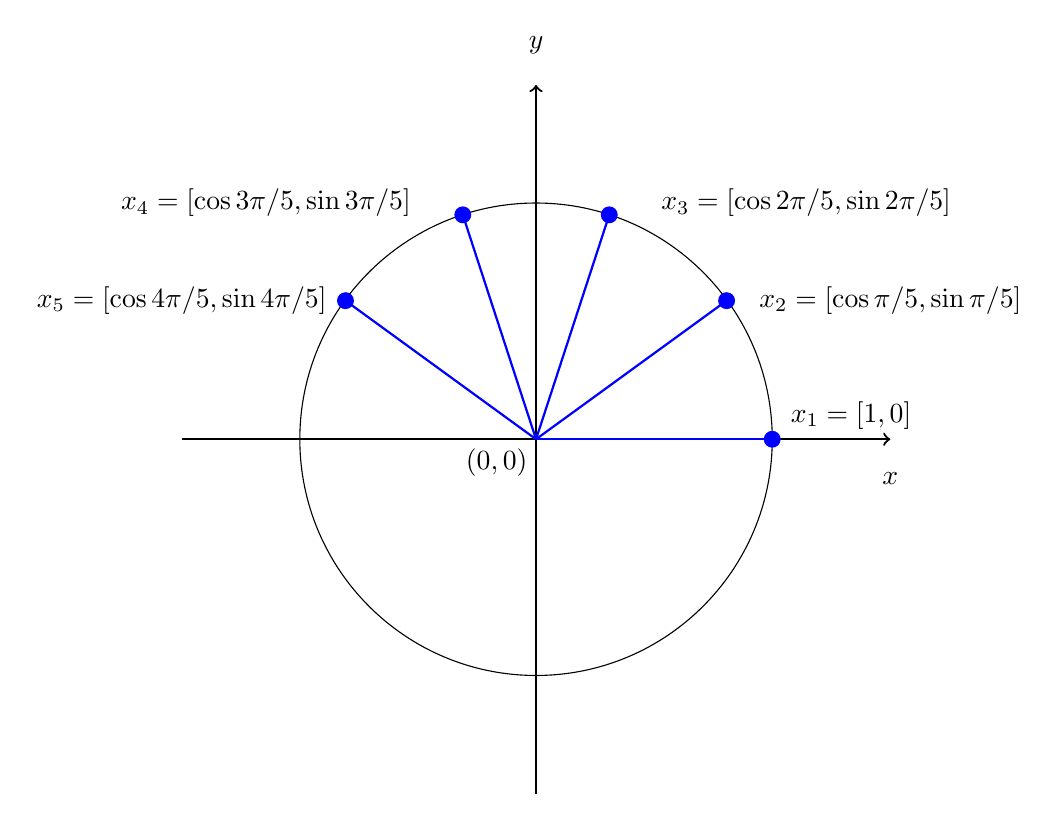
\begin{tikzpicture}[yscale=-1] 
        % x-axis
        \draw [thick,->] (-4.5, 0) -- (4.5, 0);
        % y-axis
        \draw [thick,->] (0, 4.5) -- (0, -4.5);
        % origin label
        \node at (-0.5, 0.3) {\text{$(0, 0)$}};
        % x-axis label
        \node at (4.5, 0.5) {\text{$x$}};
        % y-axis label
        \node at (0, -5) {\text{$y$}};
        % circle
        \draw (0,0) circle (3cm);
        \draw (3,0)[blue,fill=blue] circle (0.1cm);
        \draw (2.42, -1.76)[blue,fill=blue] circle (0.1cm);
        \draw (0.93, -2.85)[blue,fill=blue] circle (0.1cm);
        \draw (-2.42, -1.76)[blue,fill=blue] circle (0.1cm);
        \draw (-0.93, -2.85)[blue,fill=blue] circle (0.1cm);
        
        \draw [thick,-,blue] (3, 0) -- (0, 0);
        \draw [thick,-,blue] (2.42, -1.76) -- (0, 0);
        \draw [thick,-,blue] (0.93, -2.85) -- (0, 0);
        \draw [thick,-,blue] (-2.42, -1.76) -- (0, 0);
        \draw [thick,-,blue] (-0.93, -2.85) -- (0, 0);
        
        \node at (4, -0.3) {\text{$x_1 = [1,0]$}};
        \node at (4.5, -1.76) {\text{$x_2 = [\cos \pi/5,\sin \pi/5]$}};
        \node at (3.43, -3) {\text{$x_3 = [\cos 2\pi/5,\sin 2\pi/5]$}};
         \node at (-4.5, -1.76) {\text{$x_5 = [\cos 4\pi/5,\sin 4\pi/5]$}};
        \node at (-3.43, -3) {\text{$x_4 = [\cos 3\pi/5,\sin 3\pi/5]$}};
    \end{tikzpicture}
    \caption{A configuration of five unit vectors that produce the optimum $\epsilon$ for $n=2, N=5$}
\end{figure}

\begin{figure}[!h]
    \centering
    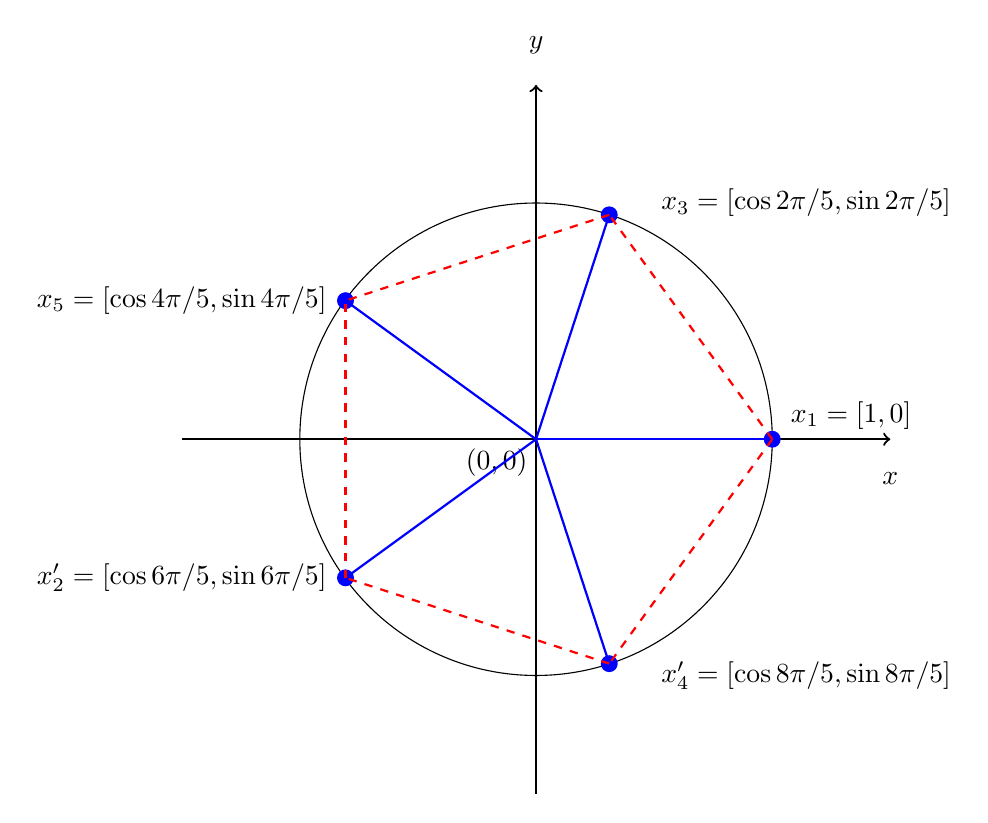
\begin{tikzpicture}[yscale=-1] 
        % x-axis
        \draw [thick,->] (-4.5, 0) -- (4.5, 0);
        % y-axis
        \draw [thick,->] (0, 4.5) -- (0, -4.5);
        % origin label
        \node at (-0.5, 0.3) {\text{$(0, 0)$}};
        % x-axis label
        \node at (4.5, 0.5) {\text{$x$}};
        % y-axis label
        \node at (0, -5) {\text{$y$}};
        % circle
        \draw (0,0) circle (3cm);
        \draw (3,0)[blue,fill=blue] circle (0.1cm);
        \draw (-2.42, 1.76)[blue,fill=blue] circle (0.1cm);
        \draw (0.93, -2.85)[blue,fill=blue] circle (0.1cm);
        \draw (-2.42, -1.76)[blue,fill=blue] circle (0.1cm);
        \draw (0.93, 2.85)[blue,fill=blue] circle (0.1cm);
        
        \draw [thick,-,blue] (3, 0) -- (0, 0);
        \draw [thick,-,blue] (-2.42, 1.76) -- (0, 0);
        \draw [thick,-,blue] (0.93, -2.85) -- (0, 0);
        \draw [thick,-,blue] (-2.42, -1.76) -- (0, 0);
        \draw [thick,-,blue] (0.93, 2.85) -- (0, 0);
        
        \node at (4, -0.3) {\text{$x_1 = [1,0]$}};
        \node at (-4.5, 1.76) {\text{$x'_2 = [\cos 6\pi/5,\sin 6\pi/5]$}};
        \node at (3.43, -3) {\text{$x_3 = [\cos 2\pi/5,\sin 2\pi/5]$}};
         \node at (-4.5, -1.76) {\text{$x_5 = [\cos 4\pi/5,\sin 4\pi/5]$}};
        \node at (3.43, 3) {\text{$x'_4 = [\cos 8\pi/5,\sin 8\pi/5]$}};
        
        \draw [thick,-,red,dashed] (3, 0) -- (0.93, 2.85);
        \draw [thick,-,red,dashed] (3, 0) -- (0.93, -2.85);
        \draw [thick,-,red,dashed] (0.93, 2.85) -- (-2.42, 1.76);
        \draw [thick,-,red,dashed] (0.93, -2.85) -- (-2.42, -1.76);
        \draw [thick,-,red,dashed] (-2.42, 1.76) -- (-2.42, -1.76);
    \end{tikzpicture}
    \caption{A configuration of five unit vectors that produce the optimum $\epsilon$ for $n=2, N=5$ with $x_2$ and $x_4$ from the previous figure reversed}
\end{figure}

Figure $3$ shows an optimum configuration for $n=2$ and $N=5$. Note by taking reflections of $x_2$ and $x_4$ in Figure $3$, we get five vectors that form a regular $5$-gon -- this can be seen in Figure $4$. A similar transformation can be done for all odd $N$; unfortunately, even $N$ cannot produce regular polygons.

\section{The Parallelogram Law}

First we give the definition of the norm on vectors in $\R^n$ in terms of the dot product:

\begin{definition}
For a vector $v\in\R^n$ the norm of $v$ is the positive value of $||v||$ given by the equation
$$
||v||^2=v\cdot v.
$$
\end{definition}
\begin{theorem}[Parallelogram Law]
For vectors $v_1,\cdots,v_n\in\R^n$, the following identity holds
$$
||v_1+\cdots+v_n||^2=\displaystyle\sum_{i=1}^n||v_i||^2+2\displaystyle\sum_{1\le i<j\le n}v_i\cdot v_j.
$$
\proof
First consider the following identity from the definition of the norm for vectors $u,v\in\R^n$:
$$
||u+v||^2=(u+v)\cdot (u+v)=u\cdot u+u\cdot v+ v\cdot u + v\cdot v=||u||^2+||v||^2+2u\cdot v.
$$
Now if we let $u=v_1$ and $v= v_2+\cdots+v_n$ we get 
$$
||v_1+v_2+\cdots+v_n||^2=||v_1||^2+||v_2+\cdots +v_n||^2+2\sum_{i=2}^n v_1\cdot v_i.
$$
If we recurse on $||v_2+\cdots +v_n||^2$ using induction we get the desired result. 
\end{theorem}


\section{$N = n+1$}
Let us consider the situation in which we try to minimize $\epsilon$ for $n+1$ vectors in an $n$ dimensional space. First we introduce the definition of a simplex, and then we will proceed to characterize $\epsilon$. 

\begin{definition}
An $n$-dimensional simplex is given by the convex hull of the $n+1$ points in $\R^{n+1}$ described as having a 1 in a single coordinate and zeros in every other coordinate. 
\end{definition}

Figure $5$ shows diagrams of a 2-dimensional simplex.

\begin{figure}[!h]
    \centering
        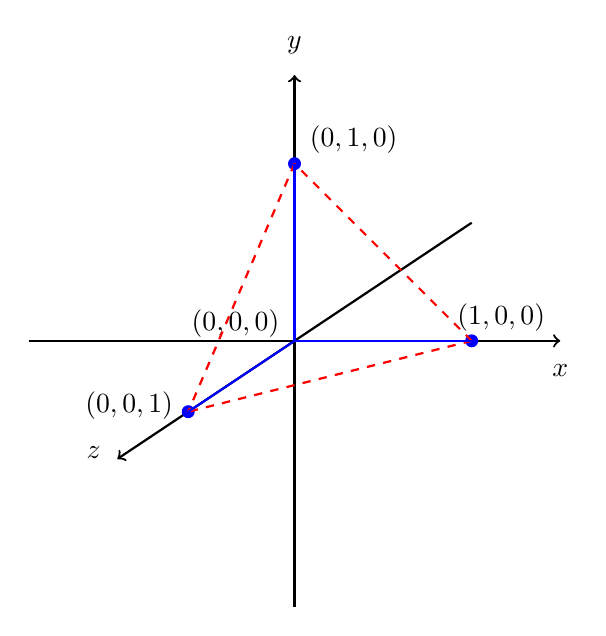
\begin{tikzpicture}[yscale=-1, scale=0.75]
        % x-axis
        \draw [thick,->] (-4.5, 0) -- (4.5, 0);
        % y-axis
        \draw [thick,->] (0, 4.5) -- (0, -4.5);
        % z-axis
        \draw [thick, ->] (3.0, -2.0) -- (-3.0, 2.0);
        % origin label
        \node at (-1, -0.3) {\text{$(0, 0, 0)$}};
        % x-axis label
        \node at (4.5, 0.5) {\text{$x$}};
        % y-axis label
        \node at (0, -5) {\text{$y$}};
         % z-axis label
        \node at (-3.4, 1.9) {\text{$z$}};
        \node at (3.5, -0.4) {\text{$(1, 0, 0)$}};
        \node at (1, -3.4) {\text{$(0, 1, 0)$}};
        \node at (-2.8, 1.1) {\text{$(0, 0, 1)$}};
        % circle
        \draw (3,0)[blue,fill=blue] circle (0.1cm);
        \draw (0, -3)[blue,fill=blue] circle (0.1cm);
        \draw (-1.8, 1.2)[blue,fill=blue] circle (0.1cm);
        
        \draw [thick,-,red,dashed] (3, 0) -- (0, -3);
        \draw [thick,-,red,dashed] (0, -3) -- (-1.8, 1.2);
        \draw [thick,-,red,dashed] (3, 0) -- (-1.8, 1.2);
        
        \draw [thick,-,blue] (3, 0) -- (0, 0);
        \draw [thick,-,blue] (0, -3) -- (0, 0);
        \draw [thick,-,blue] (-1.8, 1.2) -- (0, 0);
    \end{tikzpicture}
    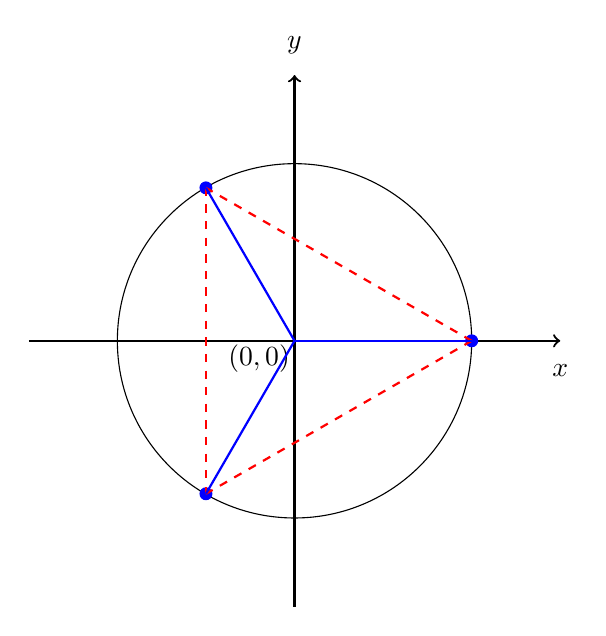
\begin{tikzpicture}[yscale=-1, scale=0.75]
        % x-axis
        \draw [thick,->] (-4.5, 0) -- (4.5, 0);
        % y-axis
        \draw [thick,->] (0, 4.5) -- (0, -4.5);
        % origin label
        \node at (-0.6, 0.3) {\text{$(0, 0)$}};
        % x-axis label
        \node at (4.5, 0.5) {\text{$x$}};
        % y-axis label
        \node at (0, -5) {\text{$y$}};
        % circle
        \draw (0,0) circle (3cm);
        \draw (3,0)[blue,fill=blue] circle (0.1cm);
        \draw (-1.5, 2.59)[blue,fill=blue] circle (0.1cm);
        \draw (-1.5, -2.59)[blue,fill=blue] circle (0.1cm);
        
        \draw [thick,-,red,dashed] (3, 0) -- (-1.5, 2.59);
        \draw [thick,-,red,dashed] (3, 0) -- (-1.5, -2.59);
        \draw [thick,-,red,dashed] (-1.5, -2.59) -- (-1.5, 2.59);
        
        \draw [thick,-,blue] (3, 0) -- (0, 0);
        \draw [thick,-,blue] (-1.5, 2.59) -- (0, 0);
        \draw [thick,-,blue] (-1.5, -2.59) -- (0, 0);
    \end{tikzpicture}

    \caption{A 2-dimensional simplex drawn in $\R^3$ on the left, and then centered at the origin in $\R^2$ on the right.}
\end{figure}

Before proceeding with the theorem, we notice that when $n=2$, the configuration of $N=3$ vectors that produced the minimum value of $\epsilon$ made up a simplex centered at the origin. 


\begin{theorem}
If $N=n+1$ and the vectors in question are denoted $v_1,\cdots, v_N$, then over all configurations of these vectors the maximum value of $v_i\cdot v_j$ for $i\neq j$ is $\frac{-1}{n}$. This is achieved when the vectors are arranged in an $n$ dimensional simplex centered at the origin, and in this configuration $\epsilon=\frac{1}{n^2}$.  
\end{theorem}

\proof
Let $\delta= \max_{i\neq j}\{v_i\cdot v_j\}$ for a given set of unit vectors $v_1, v_2, \ldots, v_{n+1}$, and let $\delta_{min}$ be the minimum possible $\delta$ obtained across all unit vectors $v_1, v_2, \ldots, v_{n+1}$. We first show that $\delta_{min} \le-\frac{1}{n}$ by showing that the origin-centered simplex configuration of the vectors $v_1,\cdots v_{n+1}$ produces a value $\delta=-\frac{1}{n}$, and then will later show that $\delta_{min} \geq -\frac{1}{n}$ as well. 

We must first describe the vectors that make up the origin centered simplex. To center our simplex at the origin we take each vector in the original simplex, and subtract from it the vector representing the centroid of the original simplex. The centroid of the original simplex takes the form $(\frac{1}{N},\frac{1}{N},\ldots,\frac{1}{N})$, so the points of the new simplex take the form
$$
\left(-\frac{1}{N},\cdots,-\frac{1}{N},\frac{N-1}{N},-\frac{1}{N},\cdots,-\frac{1}{N}\right).
$$
If we renormalize these vectors so that each vector has unit length, we get 
$$
\sqrt{\frac{N}{N-1}}\left(-\frac{1}{N},\cdots,-\frac{1}{N},\frac{N-1}{N},-\frac{1}{N},\cdots,-\frac{1}{N}\right).
$$
Now, taking the dot product between any two such vectors gives us
$$
\frac{N}{N-1}\left(-2\cdot\frac{N-1}{N^2}+(N-2)\cdot\frac{1}{N^2}\right)=\frac{N}{N-1}\cdot-\frac{1}{N}=-\frac{1}{N-1}=-\frac{1}{n}.
$$
So an upper bound on the value of $\delta_{min}$ for all configurations of $n+1$ vectors in $n+1$ dimensional space is $\frac{-1}{n}$. 

To see that $\delta_{min} \ge-\frac{1}{n}$ we use the parallelogram law.

Recall that the parallelogram law states that 

$$
||v_1+\cdots+v_{n+1}||^2=\displaystyle\sum_{i=1}^{n+1}||v_i||^2+2\displaystyle\sum_{1\le i<j\le n+1}v_i\cdot v_j.
$$
In our case we know three things. First, since the norm of any vector is greater than or equal to $0$, we can conclude that $||v_1 + \cdots + v_{n+1}||^2 \geq 0$. Second, $v_i\cdot v_j\le\delta$ for any $i<j$. Third, $||v_i||=1$. Therefore 
$$
0\le n+1+n(n+1)\delta.
$$
This implies that $\delta\ge -\frac{1}{n}$ for any set of unit vectors $v_1, v_2, \ldots, v_{n+1}$, from which we can conclude that $\delta_{min} \ge -\frac{1}{n}$ as well.

Since $\delta_{min} \le -\frac{1}{n}$ and $\delta_{min} \ge -\frac{1}{n}$, we can conclude that $\delta_{min}=-\frac{1}{n}$. From this, we can see that a $\epsilon = \frac{1}{n^2}$ is achievable for the general case of when $N=n+1$ -- this leads us to conclude that the minimum possible $\epsilon$ value for $N=n+1$ is at most $\frac{1}{n^2}$.
\section{$N>n+1$}

We conjecture that in cases where $N>n+1$ we can never have an arrangement of the vectors where all values of $|v_i\cdot v_j|^2$ are the same. Proving this remains an object of future study.

\section{Applications to sphere packing}
We should be able to prove something about the radius of spheres you can pack in the case of $N=n+1$, taking as intuition square and hexagonal tilings of the plane and cubic and tetrahedral tilings of 3-space. 

\end{document}

\usepackage{todonotes}

\newtheoremstyle{theorem}{1em}{1em}{\slshape}{0pt}{\bfseries}{.}{ }{}
\theoremstyle{theorem}
\newtheorem{theorem}{Theorem}[section]
\newtheorem*{theorem*}{Theorem}
\newtheorem{corollary}[theorem]{Corollary}
\newtheorem{proposition}[theorem]{Proposition}
\newtheorem{lemma}[theorem]{Lemma}
\newtheorem{claim}[theorem]{Claim}
\newtheorem{conjecture}[theorem]{Conjecture}
\newtheorem{definition}[theorem]{Definition}
\newtheorem*{claim*}{Claim}

\theoremstyle{remark}
\newtheorem{remark}[theorem]{Remark}
\newtheorem*{remark*}{Remark}
\newtheorem{algorithm}{Algorithm}
\newtheorem*{question*}{Question}
\newtheorem{question}{Question}
\newtheorem{example}[theorem]{Example}

\providecommand{\setN}{\mathbb{N}}
\providecommand{\setZ}{\mathbb{Z}}
\providecommand{\setQ}{\mathbb{Q}}
\providecommand{\setR}{\mathbb{R}}
\providecommand{\E}{\mathrm{E}}
\providecommand{\Pr}{\mathrm{Pr}}
\providecommand{\Var}{\mathrm{Var}}

\tikzset
{
    treenode/.style = {circle, draw=black, align=center, minimum size=1cm},
}

\makeatother

\title{Pattern Avoidance} 

\author{Yajit Jain, Deepak Narayanan, Leon Zhang}

\begin{document}

\maketitle

\section{Introduction}
In this paper we investigate pattern avoidance in finite sequences of natural numbers. We begin with an example: consider the sequences 123 and 1324. Note the order relationships of the elements of 123: we have $1< 2 < 3$. Notice in addition that there is an ordered subsequence of 1324 that follows the same general pattern, namely 124. In this situation we say that the sequence 1324 \emph{does not avoid the pattern 123}. We can also examine the sequence 1432, and observe that none of its subsequences have the same order relationships as 123. We say that 1432 \emph{avoids} 123.

With examples of a four element sequence that avoids 123 and a four element sequence that does not avoid 123, it is natural to ask the question: how many four element sequences avoid 123? And more generally, how many $n$-element sequences avoid 123? For a sequence $\pi$ that is a permutation of the elements of $\{1,\cdots,k\}$, we define
$$
s_n(\pi)=\#\{\text{the set of permutations of $\{1,\cdots, n\}$ that avoid $\pi$}\}.
$$


If we define $s_n(123)$ to be the number of $n$ element sequences that avoid 123, then the question above is equivalent to identifying the sequence $(s_n(123))_n$. In this paper we consider specific cases of a very general avoidance problem, describing the sequence $(s_n(\sigma))_n$ where $\sigma$ is any permutation of the elements of the set $\{1,2,\cdots, k\}\subset\mathbb{N}$ for some $k$.

In Sections \ref{312} and \ref{321} we consider sequences $s_n(\pi)$ where $\pi$ is an element of  \\ $\{123,132,213,231,312,321\}$, and prove the following theorem.

\begin{theorem*}
For $\pi$ in $\{123,132,213,231,312,321\}$, the sequence $(s_n(\pi))$ is the Catalan numbers.
\end{theorem*}

Of particular interest is the fact that two entirely distinct methods of proof had to be used to prove this theorem for all six permutations. In Section \ref{S4} we will consider sequences $s_n(\pi)$ where $\pi$ is a permutation of $\{1,2,3,4\}$ and state a conjecture concerning $(s_n(\pi))$. In Section \ref{Tn} we consider a variation of the avoidance problem that considers the problem of avoiding sequences in a subset $T_n$ of the permutations of $n$ elements. Before proceeding, however, we formally introduce the notation that will be used throughout this paper.  


\subsection{Notation}

\begin{definition}
A permutation of a set $D$ is a bijective map from $D$ to itself. 
\end{definition}


\begin{remark}
There are two notations for permutations, `one-line' notation and `cycle' notation. We define both below. Unless stated otherwise, we will use one-line notation in this paper.
\end{remark}

\begin{example}
Let $\pi$ be a function so that $\pi(1)=5$, $\pi(2)=4$, $\pi(3)=1$, $\pi(4)=2$, $\pi(5)=3$, and $\pi(6)=6$. Then $\pi$ is a permutation of the set $D=\{1,2,3,4,5\}$. 
\end{example}

\begin{definition}
Let $\pi$ be the permutation on elements of $\{1,2,\cdots, n\}$ so that $\pi(1)=a_1, \pi(2)=a_2,\cdots, \pi(n)=a_n$. Then in one-line notation $\pi$ is written as $\pi(1)\pi(2)\cdots\pi(n)$, or equivalently, $a_1a_2,\cdots a_n$. 
\end{definition}

\begin{example}
Using $\pi$ from the previous example, in one-line notation $\pi=541236$.
\end{example}

\begin{definition}
A cycle $(a_1\cdots a_n)$ with $1\le a_i\le n$ acts as a permutation on a sequence by sending $a_1\mapsto a_2$, $a_2\mapsto a_3$, $\cdots$, $a_n\mapsto a_1$.
\end{definition}

A more formal definition of cycle notation is especially cumbersome, so we proceed with the example above, a permutation $\pi$ with $\pi(1)=5$, $\pi(2)=4$, $\pi(3)=1$, $\pi(4)=2$, $\pi(5)=3$, and $\pi(6)=6$. To write $\pi$ in cycle notation we start with 1 and identify the cycle $1\mapsto 5\mapsto 3\mapsto 1$. Once we come back to 1 we close the cycle and write $(135)$. We keep identifying cycles until every number is accounted for. So $2\mapsto 4\mapsto 2$ gives us $(24)$ and $6\mapsto 6$ gives us $(6)$. Finally we can write $\pi$ as the composition of functions $(135)(24)(6)$. Note, cycle notation is not necessarily unique. 





\begin{definition}
The set $S_n$ is the collection of permutations of the set $\{1,2,\cdots, n\}$. 
\end{definition}

\begin{example}
$S_3=\{123,132,213,231,312,321\}$. 
\end{example}








\begin{definition}
Two finite sequences of distinct positive integers $a_1,\cdots a_k$ and $b_1,\cdots b_k$ have the same pattern (or relative order) if the $i^\text{th}$ largest entry of each unordered set $\{a_1,\cdots,a_k\}$ and $\{b_1,\cdots, b_k\}$ appears in the same position in $a_1\cdots a_k$ and $b_1\cdots b_k$ for each $1\le i\le k$. 
\end{definition}

\begin{remark}
Equivalently, two finite sequences of distinct positive integers have the same relative order if the elements in each position of the sequence satisfy the same set of inequalities.
\end{remark}

\begin{definition}
A finite sequence of distinct positive integers $a_1a_2\cdots a_n$ avoids another finite sequence of distinct positive integers $b_1\cdots b_k$ with $n\ge k$ if no subsequence $a_{i_1}a_{i_2}\cdots a_{i_k}$ of $a_1a_2\cdots a_n$ has its terms in the same relative order as $b_1\cdots b_k$. 
\end{definition}


\begin{definition} 
A permutation $\sigma\in S_n$ avoids a permutation $\pi\in S_k$ if the sequence of numbers for the one-line notation for $\sigma$ avoids the sequence of numbers for the one-line notation for $\pi$.
\end{definition}

\begin{definition}
For a permutation $\pi\in S_k$, $s_n(\pi)$ represents the number of permutations in $S_n$ that avoid $\pi$. 
\end{definition}

\emph{Yajit wrote this section. Leon closely edited this section. Deepak made minor edits to this section.}


\section{Flipping and Reversing}

In this section we will identify operations that preserve avoidance. Explicitly, we say that an operator $\mathcal{O}$ preserves avoidance if a permutation $\sigma$ avoids $\pi$ if and only if $\mathcal{O}(\sigma)$ avoids $\mathcal{O}(\pi)$. If $\mathcal{O}$ is an avoidance preserving operator then for any $\sigma\in S_k$, $s_n(\sigma)=s_n(\mathcal{O}(\sigma))$ for all $n$ and $k$. Two such operators that we will identify are the `flipping' and `reversing' operators.  

\subsection{Reversing}

We notate the reversing operator as $\mathcal{R}$. Formally, if $a_1 a_2 \ldots a_n$ is a permutation of $n$ elements, then $\mathcal{R}(a_1 a_2 \ldots a_{n-1} a_n) = a_n a_{n-1} \dots a_2 a_1$.

\begin{lemma}[Reversing Lemma]
The permutation $\sigma$ avoids the permutation $\pi$ if and only if $\mathcal{R}(\sigma)$ avoids $\mathcal{R}(\pi)$. I.e. $\mathcal{R}$ is an avoidance preserving operator. 
\end{lemma}
\begin{proof}
We need to only prove one direction of this theorem, then the other direction follows because $\mathcal{R}^2=1$. We show that if ${\sigma}\in S_n$ avoids $\pi$ then $\mathcal{R}(\sigma)$ avoids $\mathcal{R}(\pi)$. Suppose that $\mathcal{R}(\sigma)$ does not avoid $\mathcal{R}(\pi)$. Then if we reverse $\mathcal{R}(\sigma)$ again, the subsequence of $\mathcal{R}(\sigma)$ that follows the same pattern as $\mathcal{R}(\pi)$ will reverse to a subsequence that follows the same pattern as $\pi$, giving us a contradiction. Therefore $\mathcal{R}(\sigma)$ avoids $\mathcal{R}(\pi)$. 

\end{proof}

\begin{corollary} 
For a permutation $\pi$, $s_n(\pi)=s_n(\mathcal{R}(\pi))$. 
\end{corollary}
\begin{proof}
This result follows trivially because the reversing lemma describes a bijection between permutations that avoid $\pi$ and permutations that avoid $\mathcal{R}(\pi)$. 
\end{proof}

\subsection{Flipping}
In this section we introduce the concept of flipping to prove the `Flipping Lemma'.
\begin{definition}
We define the \emph{flip} of a sequence $a$ as the sequence $b$ with the same elements as $a$, but with the largest element swapped with the smallest element, the second largest element swapped with the second smallest element, etc.  The flipping operator will be denoted by $\mathcal{F}$.  
\end{definition}

\begin{example}
$\mathcal{F}(1324)=4231$.
\end{example}


\begin{lemma}[Flipping Lemma]
The permutation $\sigma$ avoids the permutation $\pi$ if and only if $\mathcal{F}(\sigma)$ avoids $\mathcal{F}(\pi)$. I.e. $\mathcal{F}$ is an avoidance preserving operator. 
\end{lemma}
\begin{proof}
Notice that we only need to prove one direction of this statement. The opposite direction will follow since applying $\mathcal{F}$ twice returns the original permutation, or $\mathcal{F}^2 = 1$. We show that if ${\sigma}\in S_n$ avoids $\pi$ then $\mathcal{F}(\sigma)$ avoids $\mathcal{F}(\pi)$. Suppose that $\mathcal{F}(\sigma)$ does not avoid $\mathcal{F}(\pi)$. Let $\mathcal{F}(\sigma)=a_1\cdots a_n$ and let $\mathcal{F}(\pi)=b_1\cdots  b_k$. Then there is some subsequence $a_{i_1}\cdots a_{i_k}$ so that $a_{i_c}<a_{i_d}$ if and only if $b_c<b_d$. Now flipping $\mathcal{F}(\sigma)$ gives us the sequence $(n+1-a_1)(n+1-a_2)\cdots(n+1-a_n)$ and flipping $\mathcal{F}(\pi)$ gives the sequence $(k+1-b_1)(k+1-b_2)\cdots(k+1-b_k)$. Thus $n+1-a_{i_c}>n+1-a_{i_d}$ if and only if $k+1-b_c>k+1-b_d$. So  this implies that $\sigma$ does not avoid $\pi$, a contradiction. 
\end{proof}

\begin{corollary} 
For a permutation $\pi$, $s_n(\pi)=s_n(\mathcal{F}(\pi))$. 
\end{corollary}
\begin{proof}
This result follows because the flipping lemma describes a bijection between permutations that avoid $\pi$ and permutations that avoid $\mathcal{F}(\pi)$. 
\end{proof}

\emph{Yajit wrote this section. Leon edited this section. Deepak made minor edits.}


\section{Avoiding Permutations of Length Three Part I}
\label{312}

We claim that the sequence of numbers $s_n(312)$ is in fact the sequence of Catalan numbers. Before formally stating and proving the result, however, we prove the following useful lemma.
\begin{lemma}
\label{lemma1}
The permutations of $\{1,2,\dots,k,k+1\}$ ending in $i$ that avoid the pattern $312$ are precisely those of the form,
$$\pi_1 \pi_2 i$$
the concatenation of $\pi_1, \pi_2$, and $i$, where $\pi_1$ is a permutation of $\{1,2,\ldots,i-1\}$ that avoids the pattern $312$ and $\pi_2$ is a permutation of $\{i+1,\ldots,k+1\}$ that avoids the pattern $312$.
\end{lemma}

\begin{proof}

It is easy to see that such a permutation is sufficient for avoiding $312$ and ending in $i$. We will prove that the condition is necessary as well.

First, we define the sets $A=\{1,2,\ldots,i-1\}$ and $B=\{i+1,i+2,\ldots,k+1\}$. For the sake of contradiction, let us assume that there exists some permutation $\pi$ of $\{1,2,...,k,k+1\}$ that ends with value $i$ such that some integer $x < i$ (that is, $x \in A$) is to the right of some integer $y > i$ ($y \in B$). Clearly, this permutation is not of the form described above, and the subsequence $(y, x, i)$ is of the same relative order as 312; as a consequence, $\pi$ does not avoid 312.

It follows that for any permutation $\pi\in S_{k+1}$ avoiding $312$ and ending in $i$, all $x < i$ must be to the left of all $y > i$. Hence $\pi$ must be the concatenation of three subsequences $\pi_1 \pi_2 i$, where $\pi_1$ is a permutation of $\{1, 2, \ldots, i-1\}$ and $\pi_2$ is a permutation of $\{i+1, i+2, \ldots, k+1\}$. Furthermore, it is clear that any subsequences of the permutation $\pi = \pi_1 \pi_2 i$ must avoid $312$ if the entire permutation $\pi$ is to avoid $312$ as well; this implies that the permutations $\pi_1$ and $\pi_2$ must avoid $312$ as well.
\end{proof}

Before we move on to the proof of our main theorem for this section, we look at the sequence of Catalan numbers.

\begin{definition}
The Catalan numbers are the sequence of positive integers $C_i$ defined as follows,
$$C_0=1, \, C_{n+1}=\sum_{i=1}^n C_iC_{n-i} \, \text{for} \; n \geq 0$$
\end{definition}

\begin{theorem}
$s_n(312), s_n(132), s_n(213)$, and $s_n(231)$ are equal to $C_n$, the $n^{th}$ Catalan number.
\end{theorem}

\begin{proof}
We prove this result for $(s_n(312))$ by induction and then use the flipping and reversing lemmas for the other three sequences. The inductive hypothesis holds for our base case of $\{1\}$, since the only permutation of $\{1\}$ trivially avoids $312$.

Let us assume that for all $i$ from $1$ to $k$, the number of permutations of $\{1,2,...,i\}$ that avoid the order $312$ as a subsequence is $C_i$.

Now, we want to prove the inductive hypothesis for $\{1,2,...,k,k+1\}$ as well. That is, we want to prove that the number of permutations of $\{1,2,...,k,k+1\}$ that avoid the order $312$ as a subsequence is $C_{k+1}$.

Using our lemma, we count the number of permutations of $\{1,2,...,k,k+1\}$ that avoid $312$ by enumerating through all possible values of the last term of a valid permutation. Consider $\pi$ a permutation of $\{1,2,\ldots, k, k+1\}$ ending in $i$. Let us define the subsets $A$ and $B$ of the  set $\{1,2,...,k+1\} \setminus \{i\}$ as the set of integers less than $i$ and the set of integers greater than $i$ respectively. It is clear from the definition of $A$ and $B$ that $A$ and $B$ are disjoint from each other.

From the above lemma, we know that all permutations of $\{1,2,...,k,k+1\}$ ending in $i$ that avoid $312$ are precisely those of the form
$$\pi = \pi_1 \pi_2 i$$
where $\pi_1$ is a permutation of $A$ that avoids $312$ and $\pi_2$ is a permutation of $B$ that avoids $312$.

It follows that the total number of permutations $\pi$ avoiding $312$ and ending in $i$ is
$$C_{i-1} \cdot C_{k-i+1},$$
since by our induction hypothesis the total number of valid choices for $\pi_1$ is simply $C_{i-1}$, and similarly the total number of valid choices for $\pi_2$ is $C_{k-1+1}$.

Now, summing over all possible values of $i$, we see that the total number of permutations of $\{1,2,...,k+1\}$ that avoid $312$ is equal to,
$$\sum_{i=1}^{k+1} C_{i-1} \cdot C_{k-i+1} = \sum_{i=0}^k C_i \cdot C_{k-i}$$ which is well-known to equal $C_{k+1}$, the $n+1$st Catalan number. The proof  therefore follows by induction.

By the flipping lemma and reversing lemma we see that  $s_n(132)$, $s_n(213)$ and $s_n(231)$ are the sequence of Catalan numbers as well. 
\end{proof}


\emph{Deepak wrote this section. Leon closely edited this section. Yajit made minor revisions.}

\section{Avoiding Permutations of Length Three Part II}

\label{321}
Unfortunately, there is no clear way to reformulate Lemma \ref{lemma1} for the case of avoiding the permutation 321 or 123. As a consequence, the proof in the previous section simply does not hold. Fortunately, however, we still have a closed form expression for $s_n(321)$ (recall that $s_n(321)=s_n(123)$ by our flipping lemma). Surprisingly, in fact, the sequence remains the same: $s_n(321)=C_n$, the $n^{th}$ Catalan number. In order to prove this result, we need the machinery of Young tableaux. What follows is a brief exposition of the key results, adapted from Chapter 8 of Stanley's \emph{Algebraic Combinatorics}.

\begin{definition}
A Young diagram of a partition $\lambda=\{\lambda_1, \lambda_2, \ldots, \lambda_n\}$ of the integer $\sum_{i=1}^n \lambda_i$ is a left-justified array of squares, with $\lambda_i$ squares in the $i$th row.
\end{definition}
\begin{example}
The Young diagram of $(4, 3, 1, 1)$ looks like:
\[
\ytableausetup{centertableaux}
\begin{ytableau}
\ & \ & \ & \ \\
\ & \ & \ \\
\ \\
\
\end{ytableau}
\]
\end{example}

\begin{definition}
A standard Young tableau (or SYT) consists of the Young diagram $D$ of some partition $\lambda$ of an integer $n$, together with the numbers $1, 2, \ldots, n$ inserted into the squares of $D$, so that each number appears exactly once, and every row and column is \emph{increasing}. We call $\lambda$ the \emph{shape} of the SYT.
\end{definition}

\begin{example}
There are five SYT of the shape $(2, 2, 1)$. They are given by
\[\ytableausetup{aligntableaux=top}
\begin{ytableau}
1 & 2 \\
3 & 4\\
5
\end{ytableau}\ \ \ \ \
\hfill
\begin{ytableau}
1 & 2 \\
3 & 5\\
4
\end{ytableau}\ \ \ \ \
\hfill
\begin{ytableau}
1 & 3 \\
2 & 4\\
5
\end{ytableau}\ \ \ \ \
\hfill
\begin{ytableau}
1 & 3 \\
2 & 5\\
4
\end{ytableau}\ \ \ \ \
\hfill
\begin{ytableau}
1 & 4 \\
2 & 5\\
3
\end{ytableau}.\]
\end{example}

\begin{definition}
Let $u$ be a square of the Young diagram of the partition $\lambda$. Then the hook $H(u)$ is the set of all squares directly to the right of $u$ or directly below $u$, including $u$ itself. The size of $H(u)$ is called the hook length of $u$, and is denoted $h(u)$.
\end{definition}

\begin{example}
In the Young diagram of the partition $(4, 2, 2)$ below, each square $u$ contains its hook length $h(u)$.
\[\ytableausetup{centertableaux}
\begin{ytableau}
6 & 5 & 2 & 1\\
3 & 2\\
2 & 1
\end{ytableau}\]
\end{example}

\begin{theorem}
Let $\lambda$ be a partition of $n$. Then $f^\lambda$, the number of SYT of shape $\lambda$, is given by
\[f^\lambda=\frac{n!}{\prod_{u\in \lambda} h(u)},\]
where the notation $u\in \lambda$ means that $u$ ranges over all squares of the Young diagram of $\lambda$.
\end{theorem}

The theorem above is called the \emph{hook-length formula}.

\begin{example}
The diagram above for the hook lengths of $\lambda=(4, 2, 2)$ tells us that the number of SYT of shape $\lambda$ is given by
\[\frac{8!}{6\cdot 5\cdot 2 \cdot 1 \cdot 3 \cdot 2 \cdot 2\cdot 1}=56.\]
\end{example}

It is an easy application of the hook-length formula to prove the following theorem:

\begin{theorem}
\label{catalan_2}
The number of SYT of shape $(n, n)$ is given by $C_n$, the $n^{th}$ Catalan number.
\end{theorem}

We need only one more result before we are ready to prove our central result.

\begin{theorem}\footnote{A more detailed exposition of this result can be found at http://math.mit.edu/~jnovak/d.18.312/lecture16.pdf. The result itself appears on page 9.}
\label{rsk}
There exists an algorithm (called the \emph{RSK algorithm}) which defines a bijection between the set of permutations in $S(n)$ avoiding a decreasing subsequence of length 3 and the set of pairs of size-$n$ SYT of the same shape and at most two rows. 
\end{theorem}
Using all this machinery and all these results, we are finally able to prove the closed-form expression for $s_n(321)$.
\begin{theorem}
$s_n(321)$ and $s_n(123)$, the number of permutations on $n$ elements which avoid 321 and 123 respectively, are equal to $C_n$, the $n^{th}$ Catalan number.
\end{theorem}
\begin{proof}
By the reversing lemma we only need to prove this result for $s_n(321)$. By Theorem \ref{rsk}, there are $s_n(321)$ elements in the set $A$ of pairs of size-$n$ SYT of the same shape and at most two rows. By Theorem \ref{catalan_2}, the set $B_n$ of SYT of shape $(n, n)$ has its size given by $C_n$. We will construct a bijection between the sets $A_n$ and $B_n$: because $|A_n|=s_n(321)$ and $|B_n|=C_n$, it will therefore follow that $s_n(321)=C_n$, as desired.

Given any pair of size $n$ Young tableaux of the same shape and at most two parts, take the second tableau and invert its numbers: that is, send $i$ to $2n+1-i$ for all $i$. Now rotate the Young tableau and `fit' it into the first tableau. We demonstrate this process for a pair of Young tableaux with $n=6$: we begin with
\[\ytableausetup{aligntableaux=top}
\begin{ytableau}
1 & 2 &3&4\\
5 & 6
\end{ytableau} \ \ \ \ \ 
\hfill
\begin{ytableau}
1 & 3 & 4 & 5\\
2 & 6
\end{ytableau}.\]
Inverting the numbers of the second tableau gives us
\[\ytableausetup{aligntableaux=top}
\begin{ytableau}
1 & 2 &3&4\\
5 & 6
\end{ytableau} \ \ \ \ \ 
\hfill
\begin{ytableau}
12 & 10 & 9 & 8\\
11 & 7
\end{ytableau}.\]
Finally, rotating the second Young tableau and fitting it into the first gives us
\[\ytableausetup{aligntableaux=top}
\begin{ytableau}
1 & 2 &3&4&7&11\\
5 & 6&8&9&10&12
\end{ytableau},\]
a valid Young tableau of shape $(6, 6)$. 

Beginning with a pair of size $n$ Young tableaux of shape $\lambda$ and at most two parts, it is easy to see that this process always yields a valid Young tableau of shape $(n, n)$. Indeed, we can define its inverse: given any Young tableau for the partition $(n, n)$, we can find the shape formed by all numbers greater than $n$: split it off from the original tableau, rotate it, and invert the numbers to get a pair of size $n$ Young tableau of the same shape and at most two parts. These processes can be easily checked to be inverses: hence the two sets are of the same size, and the proof follows.
\end{proof}

\emph{Leon wrote this section. Yajit made minor revisions.}

\section{Conjectures on $s_n(\pi)$ for $\pi\in S_4$}
\label{S4}


In this section we present our findings and conjectures about sequences $s_n(\pi)$ for $\pi\in S_4$. Using the flipping and reversing operators we can group elements of $S_4$ by their orbits. The following groups appear: 
$$
\{1234,4321\},
\{1243,4312,2134,3412\},
\{1432,4123,2341,3214\},
\{2143,3412\},
$$
$$
\{4132,1423,2314,3241\},
\{4213,1342,3124,2431\},
\{2413,3142\},
$$
$$
\{4231,1324\}
$$
So all permutations that belong to a single group in the list above must produce the same sequence. 
We computed values up to $s_{9}$. It appears that there are three sequences that appear, and we have sorted the permutations according to which sequence they produce and paired them with their flips.  



We define the following sequences based on the first nine terms:
$$
A:=1,2,6,23,103,512,2740,15485,91245\ldots
$$
$$
B:=1,2,6,23,103,513,2761,15767,94359\ldots
$$
$$
C:=1,2,6,23,103,513,2762,15793,94776\ldots
$$

The table below lists the elements of $S_4$ generate sequences $A,B,C$ for the first 8 terms.

\begin{center}
\begin{tabular}{|c|c|c|}
B &A&C\\
\hline
1234, 4321&4132, 1423&4231, 1324\\
1243, 4312&4213, 1342&\\
1432, 4123&2431, 3124&\\
2134, 3421&2413, 3142&\\
2143, 3412&2314, 3241&\\
2341, 3214&&\\
\end{tabular}
\end{center}

Comparing this table to the orbit decomposition above we notice that all of the groups in the first line appear to produce sequence $B$, all of the groups in the second line appear to produce sequence $A$, and the single orbit in line three produces sequence $C$. There is no guarantee that these sequences will not diverge and produce more than three distinct sequences, however for now we hypothesize that $A$, $B$, and $C$ are the only sequences that arise for $s_n(\pi)$ with $\pi\in S_4$. Assuming this hypothesis, if we write each length four permutation in cycle notation, a pattern begins to emerge. 

\begin{center}
\begin{tabular}{|c|c|c|}
B &A&C\\
\hline
(1)(2)(3)(4),(14)(23)&(243),(142)&(23),(14)\\
(34),(1423)&(234),(143)&\\
(24),(1432)&(124),(132)&\\
(12),(1324)&(123),(134)&\\
(12)(34),(13)(24)&(1243),(1342)&\\
(1234),(13)&&\\
\end{tabular}
\end{center}

So we conjecture that sequence $A$ is characterized by elements of $S_4$ that are three cycles or four cycles when written in cycle notation. Sequence $B$ seems to be characterized by either a pair of disjoint two cycles paired with a flip that is a pair of disjoint 2-cycles, or a single 4-cycle paired with a flip that is a 2-cycle. Sequence $C$ appears to be characterized by a 2-cycle paired with a 2-cycle as a flip. 

\

\emph{Yajit wrote this section. Leon edited this section.}

\section{Avoidance of Permutations of $T_n$}
\label{Tn}
We now impose further restrictions on the set of permutations $S_n$. This new set of permutations, $T_n$ is defined as follows.

\begin{definition}
Let $n$ be an even integer. The set $T_n$ is defined as the set of all permutations $\sigma \in S_n$ in which $1,3,5,\ldots,2n-1$ appear in increasing order, and $2i$ always appears to the right of $2i-1$.
\end{definition}

Since $T_n$ is only defined for even $n$, wherever convenient, we shall refer to $T_n$ as $T_{2m}$ where $m$ is any integer greater than or equal to $1$.

Given the above definition of $T_{2m}$, we prove the following result about the cardinality of $T_{2m}$.

\begin{theorem}
$|T_{2m}| = 1 \cdot 3 \cdot 5 \cdot \ldots \cdot (2m-1)$
\end{theorem}

\begin{proof}
Because $1,3,5,\ldots,2m-1$ must appear in increasing order in $T_{2m}$, the size of $T_{2m}$ is given by the number of ways in which $2, 4, 6, \ldots, 2m$ can be ordered relative to each other and to $1, 3, \ldots, 2m-1$.

Let us first insert $2m$ into the sequence $1,3,5,\ldots,2m-1$. Because $2m$ must appear to the right of $2m-1$, it can be inserted into only a single slot, the one following $2m-1$. (By ``slot'' we mean a gap between two existing elements of the sequence, or the gap that follows the last element of the sequence, or the gap that precedes the first element of the sequence.)

Next let us insert $(2m-2)$ into the sequence. $(2m-2)$ can be inserted into $3$ slots in the sequence -- the one between $2m-3$ and $2m-1$, the one between $2m-1$ and $2m$ or the one following $2m$.

We want to next insert $(2m-4)$ into this incompletely formed sequence; we see that there are $5$ possible locations. Continuing this for all even numbers up to $2$, we observe that the total number of ways such a sequence can  be created is equal to $1 \cdot 3 \cdot 5 \cdot \ldots \cdot (2m-1)$, as desired.
\end{proof}

We will now study avoidance of permutations in $T_n$. In this section, we consider the sequence of numbers $t_n(\pi)$, defined as 
\[t_n(\pi)=\#\{\sigma\in T_n|\sigma \text{ avoids } \pi\},\]
with $\pi\in S_3$.

Before stating our conjectures, we present the computed sequences. Note that since the sequence $T_n$ is defined only for even $n$, we only present the even terms of the sequence $t_n$.

$$t_n(123) = 1, 0, 0, 0, 0, \ldots$$
$$t_n(132) = 1, 1, 1, 1, 1, \ldots$$
$$t_n(213) = 1, 2, 4, 8, 16, \ldots$$
$$t_n(231) = 1, 2, 4, 8, 16, \ldots$$
$$t_n(312) = 1, 3, 12, 55, 273, \ldots$$
$$t_n(321) = 1, 3, 12, 55, 273, \ldots$$

It is easy to see why $t_n(123)$ and $t_n(132)$ behave the way they do -- since all odd numbers in $T_n$ are increasing, it is impossible to have a permutation in $T_n$ that avoids $123$ and the permutation consisting of all increasing integers is the only permutation of $T_n$ that avoids $132$.

More interesting are the equivalences between $213$ and $231$, and $312$ and $321$. We  prove the equivalence between $312$ and $321$ below, but before doing so, we first state and prove the following useful lemmas.

\begin{lemma}
\label{tn_avoidance}
Let $a$ and $b$ be two elements that appear in a permutation in $T_n$ such that $a$ is to the left of $b$. If $a > b$, then $b$ must be even.
\end{lemma}

\begin{proof}
For the sake of contradiction, let us assume that $b$ is odd. Then there exist two possibilities that need to be considered -- either $a$ is odd or $a$ is even.

\begin{itemize}
\item \textbf{Case 1:} $a$ is odd.

Note that all permutations in $T_n$ must have odd elements monotonically increasing. So if $a$ appears to the left of $b$, and both $a$ and $b$ are odd, then $a$ must be less than $b$ -- a contradiction. Hence $a$ cannot be odd.

\item \textbf{Case 2:} $a$ is even.

For all permutations $\sigma$ in $T_n$, every even element $j$ must be to the right of all odd elements less than $j$. Since $a$ is even, therefore, it must be to the right of all odd numbers less than it. But $b$ is an odd number less than $a$, and $a$ is to the left of $b$ -- another contradiction. Hence $a$ cannot be even, either.
\end{itemize}

We conclude that $b$ must be even, as desired.
\end{proof}

\begin{lemma}
\label{swapping_lemma}
If $x, y, z$ is a three-element subsequence of a permutation $\pi$ in $T_n$ such that $x > y > z$ or $x > z > y$, then swapping $y$ and $z$ in the permutation $\pi$ yields a permutation that also belongs to $T_n$.
\end{lemma}

\begin{proof}
Since $x$ is to the left of $y$ and $z$, and $x>y$ and $x>z$, it follows by Lemma \ref{tn_avoidance} that both $y$ and $z$ must be even. Let $\pi'$ be the permutation obtained by swapping $y$ and $z$ in the permutation $\pi$. We divide our analysis into two cases:
\begin{itemize}
\item \textbf{Case 1:} $x$ is odd.

Then it suffices to check that $y$ is to the right of $y-1$ and that $z$ is still to the right of $z-1$. This is easy: since $y-1$ and $z-1$ are odd numbers less than $x$ (another odd number, by assumption), they must be to the left of $x$, and hence to the left of $y$ and $z$.

\item \textbf{Case 2:} $x$ is even.

Since $\pi\in T_n$, $x-1$ must be to the left of $x$. Because $x>y$ and $x>z$, we must have that $x-1>y-1$ and $x-1>z-1$. It follows that $y-1$ and $z-1$ are to the left of $x-1$, and hence $x$, in $\pi$. We conclude that $y$ and $z$ are to the right of $y-1$ and $z-1$ in $\pi'$, since $y-1$ and $z-1$ are to the left of $x$ and $y$ and $z$ remain to the right of $x$.
\end{itemize}
Hence, regardless of the parity of $x$, swapping $y$ and $z$ yields a permutation $\pi'$ that also belongs to $T_n$, as desired.
\end{proof}

With these lemmas in hand, we now present a proof that $t_n(312) = t_n(321)$.

\begin{theorem}
There exists a bijection between the set of permutations in $T_n$ avoiding 312 and the set of permutations in $T_n$ avoiding 321. As a consequence, $t_n(312)=t_n(321)$.
\end{theorem}

\begin{proof}
Let $A$ be the set of permutations in $T_n$ avoiding 312, and $B$ the set of permutations in $T_n$ avoiding 321. Let $a$ be an arbitrary permutation in $A$, and $b$ an arbitrary permutation in $B$. By the definition of $A$, $a$ avoids 312. Pick any positive integer $i\leq n$. We note that all even integers to the right of $i$ and less than $i$ in $a$ must be in decreasing order; otherwise, we would obtain a subsequence with pattern 312. Similarly, all even integers to the right of $i$ and less than $i$ in $b$ must be in increasing order.

In fact, note that any permutation $\pi\in T_n$ which satisfies this condition - for all $i\leq n$, all the even integers to the right of $i$ and less than $i$ are in decreasing order - is a permutation in $A$. Suppose for the sake of contradiction $\pi$ had a subsequence $x, y, z$ following the pattern 312 (so in particular $x>z>y$). Since it is in $T_n$, by Lemma  \ref{tn_avoidance} $y$ and $z$ must be even. Then by the assumed property of $\pi$ we must have $y>z$, a contradiction; hence such a subsequence cannot exist, and so $\pi$ avoids 312. We have a similar result for $B$: $B$ is precisely the set of permutations $\pi\in T_n$ satisfying the condition that, for all $i\leq n$, all even integers to the right of $i$ and less than $i$ are in decreasing order.

Then the bijection between $A$ and $B$ is as follows: given a permutation $a\in A$, consider each of its elements $i$ beginning with its rightmost element and moving leftward. By the argument above, the collection of even elements to the right of $i$ and less than $i$ will be in decreasing order; for each $i$, we sort this collection to make the elements increasing instead. Note that this process can be obtained by transposing elements, so that by Lemma \ref{swapping_lemma} the result at each stage will be a permutation in $T_n$. The end result will therefore be a permutation in $T_n$ with the property that for each $i$, all even integers to the right of $i$ and less than $i$ must be in increasing order. As we argued above, therefore, the end result is a permutation in $B$.

Indeed, it is easy to see that this process is invertible: for each element $j$, beginning with the leftmost element and moving right, we reverse sort the elements less than $j$ and to the right of $j$. Since the process is invertible, this map in fact defines a bijection, as desired.
\end{proof}

Unfortunately, it turns out that proving the equivalence between $231$ and $213$ is not as straightforward as above. In fact, however, we can prove a stronger result: both $t_n(231)$ and $t_n(213)$ are equal to $2^{n/2-1}$, and hence the sequences we obtain are equivalent.

\begin{theorem}
$t_n(231)$, the number of permutations in $T_n$ avoiding the pattern 231, where $n$ is even, is equal to $2^{n/2-1}$.
\end{theorem}

\begin{proof}
Let $n=2m$. Consider a permutation $\sigma$ in $T_{n}$ that avoids $231$, and consider an arbitrary even element $2i$ in $\sigma$. For this element $2i$, define $A$ to be the set of numbers greater than $2i$ and to its left in the permutation $\sigma$. First off, we claim that the set $A$ cannot contain any even numbers. To see why, suppose for the sake of contradiction that there existed such an even number $a$. Then $a-1$ would be to the left of $a$, because $\sigma\in T_{2m}$, and $a-1>2i$, so that $a-1, a, 2i$ is a subsequence with pattern 231: a contradiction.

Furthermore, the set $A$ cannot contain any odd elements greater than $2i+1$. To see why, again suppose such an element $2j+1$ existed. Then $2i+1$ would appear to the left of $2j+1$, since our permutation $\sigma\in T_{2m}$, and so $2i+1, 2j+1, 2i$ would be a subsequence with pattern 231: again a contradiction.

It follows from these two results that the only elements to the left of $2i$ must be either less than $2i$ or $2i+1$. We claim that each even $2i$ can appear only in the $2i$ or $2i+1$st index, and that $2i+1$ appears in the other index. To prove this, we induct on $i$. First, we address the base case: $i=1$. Since the first entry must be 1, and the only elements which can appear to the left of 2 are 1 and 3, 2 must either be in the second or third entry; furthermore, it is clear that 3 must appear in the other entry. The base case therefore follows.

Now suppose the claim holds up to some general $i-1$. We want to show that it holds for $i$ as well. By the argument at the beginning of the proof, there are only $2i$ elements which can appear to the left of $2i$, so that the largest index in which $2i$ can appear is $2i+1$. By the induction hypothesis, however, the earliest index in which $2i$ can appear is $2i$: all the earlier indices have already been occupied. As in the base case, it is easy to see that if $2i$ is in the $2i$th position, then $2i+1$ must be in the $2i+1$st position, and if $2i$ is in the $2i+1$st position, then $2i+1$ must be in the $2i$th index. The claim follows by induction

Combining all these facts together, we see that the number of permutations $\sigma$ in $T_{2m}$ that avoid $231$ must be equal to $ 2^{m-1} = 2^{n/2-1}$, since every even element except $2m$ can be inserted in exactly two positions in $\sigma$.

\end{proof}

\begin{theorem}
$t_n(213)$, the number of permutations in $T_n$ avoiding the pattern 213, where $n$ is even, is equal to $2^{n/2-1}$.
\end{theorem}

\begin{proof}
Let $n=2m$. We first define $A_m$ as the set of all permutations in $T_{2m}$ that avoid $213$. It is easy to see that $t_m(213)$ is simply the size of $A_m$.

We claim that for every permutation $\sigma$ in $A_m$, the numbers $2m-1$ and $2m$ must be consecutive in the permutation $\sigma$. We prove the claim by contradiction: suppose otherwise, i.e. that $2m-1$ and $2m$ are not consecutive in our arbitrary choice of $\sigma$. Then there must exist some $j$ between them, and $2m-1, j, 2m$ is clearly a subsequence following the pattern 213, a contradiction. Hence $2m-1$ and $2m$ must be consecutive.

We prove the theorem by induction on $m$. That is, we prove that the size of $A_m$ is precisely $2^{m-1}$. First, we easily see that $A_1$ has only one element, so that the base case holds.

Suppose the induction hypothesis holds up to some general $m-1$, i.e. that $A_{m-1}$ has size $2^{m-2}$. We see that we can construct $A_m$ from $A_{m-1}$ by inserting the consecutive elements $2m-1, 2m$ into a permutation $\sigma'$ in $A_{m-1}$. We claim that we get a valid permutation $\sigma$ in $A_m$ from $\sigma'$ only if we insert the consecutive elements $2m-1, 2m$ right after either $2m-3$ or $2m-2$ in $\sigma'$ (which themselves are consecutive in $\sigma'$ from the above claim).

First, note that $2m-1, 2m$ must be inserted to the right of  $2m-3$, because of the way $T_{2m}$ is defined. Furthermore, if we insert $2m-1, 2m$ right after some $a$ in $\sigma$ not equal to $2m-3$ or $2m-2$, then we see that the produced permutation $\sigma$ has a three-element sub-sequence in the relative ordering $213$ -- $(2m-2, a, 2m-1)$. Hence we conclude that $2m-1, 2m$ must be inserted to the right of either $2m-3$ or $2m-2$; since we can do this for every permutation $\sigma'$ in $A_{m-1}$, we conclude that $|A_m| = 2|A_{m-1}|$. By the induction hypothesis, we have that $|A_{m-1}|=2^{m-2}$: so $A_m$ has size $2^{m-1} = 2^{n/2 - 1}$, as desired, and the result follows by induction.
\end{proof}

\

\emph{Deepak wrote this section. Leon rewrote parts of it. Yajit closely edited this section.}

\end{document}